\documentclass[11pt]{report}
\usepackage{graphics}
\usepackage{graphicx}
\usepackage{epsfig}
\usepackage{fancyhdr}
\usepackage{fullpage}
\usepackage{epsfig}
\usepackage{tabularx,ragged2e,booktabs,caption}
\usepackage{algorithm}
\usepackage{algorithmic}
\usepackage{tocloft}
\usepackage[bookmarks=false]{hyperref}
\usepackage{graphicx}
\usepackage{tikz}

\newcommand{\SubItem}[1]{
    {\setlength\itemindent{15pt} \item[-] #1}
}

\usetikzlibrary{shapes.misc, positioning}

\usetikzlibrary{shapes.geometric, arrows}
\definecolor{orange}{HTML}{eeeeee}

\tikzstyle{process} = [rectangle, minimum width=4.4cm, minimum height=1cm, text centered, draw=black, fill=orange]
\tikzstyle{process1} = [rectangle, rounded corners=0.5cm, minimum width=6cm, minimum height=1.5cm, text centered, draw=black, fill=orange, align=center]
\tikzstyle{process2} = [ font=\small, rectangle, rounded corners=0.5cm, minimum width=3cm, minimum height=1.5cm, text centered, draw=black, fill=orange, align=center]
\tikzstyle{oval} = [ellipse, minimum width=3cm, minimum height=2cm, text centered, draw=black, fill=orange]
\tikzstyle{oval2} = [ellipse, minimum width=2cm, minimum height=1.5cm, text centered, draw=black, fill=orange]

\tikzstyle{func} = [rounded rectangle]
\tikzstyle{arrow} = [thick,->,>=stealth]
\tikzstyle{overlay} = [dashed, rectangle, text centered, draw=black, align=center]


\newlength{\mylen}
\renewcommand{\cftfigpresnum}{\figurename\enspace}
\renewcommand{\cftfigaftersnum}{:}
\settowidth{\mylen}{\cftfigpresnum\cftfigaftersnum}
\addtolength{\cftfignumwidth}{\mylen}

\renewcommand{\cfttabpresnum}{\tablename\enspace}
\renewcommand{\cfttabaftersnum}{:}
\settowidth{\mylen}{\cfttabpresnum\cfttabaftersnum}
\addtolength{\cfttabnumwidth}{\mylen}


\begin{document}
\renewcommand\bibname{References}
\pagestyle{fancy}
\fancyhead{}
\fancyfoot{}
\fancyfoot[c]{\thepage}
\fancyfoot[l]{Dept. of Computer Engineering, MEC, 2019}
\lhead{abcd}
\renewcommand{\chaptermark}[1]{
\markboth{\thechapter.\ #1}{}} 
\renewcommand{\headrulewidth}{0.1pt}
\fancyhead[r]{\slshape \leftmark}
\addtolength{\headheight}{\baselineskip}
\addtolength{\headsep}{.1in}
\lhead{\nouppercase{\rightmark}}
\rhead{\nouppercase{\leftmark}}
\lhead{MultiFrame Hand Gesture GUI Control System using Convex Hull Algorithm}

\begin{titlepage}
\begin{center}

\Huge{\textbf{MultiFrame Hand Gesture GUI Control System using Convex Hull Algorithm}}\\
\vspace{0.05in}
\large{\textbf{CS451 Project\\}}
\vspace{1.2in}

\Large{\textbf{MDL15CS002 CSU 151 19}}	\hspace{.1in}	\Large{\textbf{GEORGE THOMAS SHANTI}}\\ 
\Large{\textbf{MDL15CS003 CSU 151 46}}	\hspace{.1in}	\Large{\textbf{PRINCE MATHEW}}\\ 
\Large{\textbf{MDL15CS025 CSU 151 51}}	\hspace{.1in}	\Large{\textbf{RIZA SALAHUDDIN}}\\ 
\Large{\textbf{B. Tech Computer Science \& Engineering}}


\vspace{1in}
\begin{figure}[h]
\begin{center}

\epsfig{width=1.3in, file=logo.jpg}
% If you have access to better quality logo image, that may be used, but all the groups should use the same image
\end{center}
\end{figure}
%\vspace{.2in}
\textbf{
Department of Computer Engineering\\
Model Engineering College\\
Thrikkakara, Kochi 682021\\
Phone: +91.484.2575370\\
http://www.mec.ac.in \\
hodcs@mec.ac.in\\
\vspace{0.2in}
{\upshape April 2019}
}
\end{center}
\end{titlepage}




\begin{titlepage}
\begin{center}
\Large{\textbf{Model Engineering College Thrikkakara}}\\
\Large{\textbf{Department of Computer Engineering}}\\
\end{center}
\begin{figure}[h]
\begin{center}

\epsfig{width=1.2in, file=logo.jpg}
\end{center}
\end{figure}
\begin{center}
\Large{\textbf{C E R T I F I C A T E}}\\
\vspace{.1in}
\end{center}
This is to certify that, this report titled \textbf{\textit{MultiFrame Hand Gesture GUI Control System using Convex Hull Algorithm}} is a bonafide record of the work done by\\
\\
\Large{\textbf{MDL15CS002 CSU 151 19}}	\hspace{.1in}	\Large{\textbf{GEORGE THOMAS SHANTI}}\\ 
\Large{\textbf{MDL15CS003 CSU 151 46}}	\hspace{.1in}	\Large{\textbf{PRINCE MATHEW}}\\ 
\Large{\textbf{MDL15CS025 CSU 151 51}}	\hspace{.1in}	\Large{\textbf{RIZA SALAHUDDIN}}\\ 
\\
\normalsize
\centerline  {\textsf{Eighth Semester B. Tech. Computer Science \& Engineering}}\\
students,  for the course work in \textbf{CS451 Project}, which is the second part of the two semester project work, under our guidance and supervision, in partial 
 fulfillment of the requirements for the award of the degree, B. Tech. Computer 
Science \& Engineering of \textbf{APJ Abdul Kalam Technological University}.

\footnotesize
\vspace{.1in}
\begin{tabbing}
xxxxxxxxxxxxxxxxxxxxxxxxxxxxxxxxxxxxxxxxxxxxxxx\= xxxxxxxxxxxxxxxxxx\= \kill

Guide		\>				
\\
\\
\\
Sheena K.V \>\>\\
Assistant Professor	\>\>\\
Computer Engineering	\>\>	
\end{tabbing}
\vspace{.1in}
\begin{tabbing}
xxxxxxxxxxxxxxxxxxxxxxxxxxxxxxxxxxxxxxxxxxxxxxx\= xxxxxxxxxxxxxxxxxx\= \kill

Coordinator\>\> Head of the Department
\\
\\
\\
Dr. Priya S \>\>Manilal D L\\
Associate Professor	\>\> Associate Professor\\
Computer Engineering	\>\>	Computer Engineering
\end{tabbing}
\vspace{.08in}
%
\begin{tabbing}
xxxxxxxxxxxxxxxxxxxxxxxxxxxx\= xxxxxxxxxxxxxxxxxx\= \kill
%			\>Head of the Department \\
\\
\\
\today
%\>Ahammed Siraj K K\\
%\>Associate Professor\\
%\>Computer Engineering\\
\end{tabbing}

\end{titlepage}


\begin{titlepage}
\vspace{.25in}	
\begin{center}
\textbf{Acknowledgements}\\
\end{center}
\normalsize

This project would not have been possible without the kind support and help of many individuals. We would like to extend my sincere thanks to all of them.
  
First of all, We would like to thank our esteemed Principal, Prof. (Dr.) V.P Devassia, for his guidance and support in maintaining a calm and refreshing environment to work in and also for providing the facilities that this work demanded.
  
We am highly indebted to our Project Coordinator, Dr. Priya S, Associate Professor and Head of the Department, Dr. Manilal D L, Associate Professor for their guidance, support and constant supervision throughout the duration of the work as well as for providing all the necessary information and facilities that this work demanded.

We would like to thank our Project Guide, ..... for his/her support and valuable insights and also for helping me out in correcting any mistakes that were made during the course of the work. 
  
We offer our sincere gratitude to all our friends and peers for their support and encouragement that helped me get through the tough phases during the course of this work.
  
Last but not the least, we thank the Almighty God for guiding me through and enabling us to complete the work within the specified time.
\vspace{.25in}

\vspace{.25in}


\flushleft \small{\texttt{George Thomas Shanti}}
\flushleft \small{\texttt{Prince Mathew}}
\flushleft \small{\texttt{Riza Salahuddin}}
 
\end{titlepage}



\begin{abstract}
\pagenumbering{roman}

The proposed system will allow users to manipulate his operating system’s GUI with his/her hands to do virtually anything. From moving around elements on the GUI such as windows and manipulating them to zooming in on pages, rotating them and using your hands as your own custom cursor. The research effort centralizes on the efforts of implementing an application that employs computer vision algorithms and gesture recognition techniques which in turn results in developing a low cost interface device for interacting with objects in virtual environment using hand gestures.
\end{abstract}

\tableofcontents

\cleardoublepage

\addcontentsline{toc}{chapter}{\listfigurename}
\listoffigures

\cleardoublepage

\addcontentsline{toc}{chapter}{\listtablename}
% \listoftables
 
\newpage

\pagenumbering{arabic}
\chapter{Introduction}

For decades the mouse and keyboard have been the primary choice of input device to use computers. We propose a complete methodology of controlling the operating system using fluid natural of hand gestures using the normal web camera instead of the conventional mouse. This can have wide range of applications.

Evolution of ubiquitous computing, current user interaction approaches with keyboard, mouse and pen are not sufficient for the still widening spectrum of Human computerinteraction. Gloves and sensor based trackers are unwieldy,constraining and uncomfortable to use. Due to the limitation of these devices the useable command set based diligences isalso limited. Direct use of hands as an input device is an innovative method for providing natural Human Computer Interaction which has its inheritance from textbased interfaces through 2D graphical-based interfaces, multimedia-supported interfaces, to full-fledged multiparticipant Virtual Environ-
ment (VE) systems. The proposed system will allow users to
manipulate his operating system’s GUI with his/her hands to do virtually anything. From moving around elements on the GUI such as windows and manipulating them to zooming in on pages, rotating them and using your hands as your own custom cursor. The research effort centralizes on the efforts of implementing an application that employs computer vision algorithms and gesture recognition techniques which in turn results in developing a low cost interface device for interacting with objects in virtual environment using hand gestures.

The prototype architecture of the application comprises of a central computational module that applies the brute force matching technique for tracking of hands and its gestures. Haar like technique has been utilized as a classifier that is creditworthy for locating hand position and classifying gesture. The patterning of gestures has been done for recognition by mapping the number of defects that is formed in the hand with the assigned gestures. The virtual objects are produced using Open GL library. This hand gesture recognition technique
aims to substitute the use of mouse for interaction with the
virtual objects. This will be useful to promote controlling applications like virtual games, browsing images etc in virtual
environment using hand gestures.

\section{Proposed Project}

\subsection{Problem Statement}

The existing Hand Gesture Recognition systems recognize only single frame hand gestures and are not 
responsive. The better systems which track such movement require special hardwares which are very costly.
The existing Mouse/Keyboard combination of input is lacking in fluidity of motion.

\subsection{Proposed Solution}
The proposed solution is developing a system called "MultiFrame Hand Gesture GUI Control System using Convex Hull Algorithm"
which uses the standard webcam built in laptops to record multiple frame hand gestures and execute corresponding GUI commands in the OS.


\chapter{System Study Report}
\section{Literature Survey}
\begin{enumerate}
    \item K. Oka, Y. Sato, “Real-Time Fingertip Tracking and Gesture Recognition - Their method uses a filtering technique, in addition to detecting fingertips  in  each  image  frame,  to predict fingertip locations in successive image frames and to examine the correspondences between the predicted locations and detected fingertips. This lets us obtain multiple fingertips’ trajectories in real time and improves fingertip tracking. This method can track multiple fingertips reliably even on a complex background under changing lighting conditions without invasive devices or color markers.
    
    \item Lai, H. Y., Lai, H. J., Real-Time Dynamic Hand Gesture Recognition - The  eleven  kinds  of  hand  gestures have  been  dynamic  recognized,  which  represent  the  number from  one  to  nine.  The  dynamic  images  are  caught  by  a  dynamic video.  We  use  the  YCbCr  color  space  transformation  to  detect the  skin  color  and  to  find  the  hand  contour from  the  complex background. Convex defect character points of the hand contour are  defined,  and  the  finger  angles  and  fingertip  positions  are calculated to recognize the hand gestures. The OpenCV is used to perform our research. Ten tested users produce 330 cases to recognize  eleven  hand  gestures,  and  each  hand  gestures  have  three different poses of hand gestures.  The accurate recognition rate is 95.1\%.

    \item Z. Ren, J. Yuan, J. Meng , Z. Zhang, Robust Part-Based Hand Gesture Recognition Using Kinect Sensor -The recently developed depth sensors, e.g., the Kinect sensor, have provided new opportunities for human-computer interaction (HCI). Although great progress has been made by leveraging the Kinect sensor, e.g., in human body tracking, face recognition and human action recognition, robust hand gesture recognition remains an open problem. Compared to the entire human body, the hand is a smaller object with more complex articulations and more easily affected by segmentation errors. It is thus a very challenging problem to recognize hand gestures. This paper focuses on building a robust part-based hand gesture recognition system using Kinect sensor. To handle the noisy hand shapes obtained from the Kinect sensor, we propose a novel distance metric, Finger-Earth Mover's Distance (FEMD), to measure the dissimilarity between hand shapes. As it only matches the finger parts while not the whole hand, it can better distinguish the hand gestures of slight differences. The extensive experiments demonstrate that our hand gesture recognition system is accurate (a 93.2\% mean accuracy on a challenging 10-gesture dataset), efficient (average 0.0750 s per frame), robust to hand articulations, distortions and orientation or scale changes, and can work in uncontrolled environments (cluttered backgrounds and lighting conditions) 
    
    \item Ji-Hwan Kim,Nguyen Duc Thang,Tae-Seong Kim, 3-D Hand Motion Tracking and Gesture Recognition Using a Data Glove- Developed a 3-D hand motion tracking and gesture recognition system via a data glove (namely the KHU-l data glove consisting of three tri-axis accelerometer sensors, one controller, and one Bluetooth). The KHU-l data glove is capable of transmitting hand motion signals to a PC through wireless communication via Bluetooth. Also we have implemented a 3-D digital hand model for hand motion tracking and recognition. The implemented 3-D digital hand model is based on the kinematic chain theory utilizing ellipsoids and joints. Finally, we have utilized a rule-based algorithm to recognize simple hand gestures namely scissor, rock, and paper using the 3-D digital hand model and the KHU-l data glove.
    
    \item Takuro Niidome, Rokuya Ishii, A GUI Support System for a Sight Handicapped Person By Using Hand Shape Recognition - A GUI Support System for a Sight Handicapped Person By Using Hand Shape Recognition - An algorithm of hand-shape recognition and applies to a Graphical User Interface (GUI) support system for a sight handicapped person. This algorithm is to recognize the angle of a hand and ten hand-shapes. As one application of this algorithm, we implement a system in which the angle of a hand controls a reading point in a text on a screen in real time, and a text is read out with a sound syntheses software. Further, in this system, more complicated directions to control a text reader can be done by recognized hand-shapes
    
    \item X. Wu, C. Yang, Y. Wang, H. Li, and S. Xu, “An Intelligent Interactive System Based on Hand Gesture Recognition Algorithm and Kinect,” - A cascade control algorithm integrating electromyography bio-feedback into hand gesture recognition is proposed. The outer loop is the trajectory motion tracking with Kinect-based gesture decoding classifier, and the inner loop is torque control with electromyography bio-feedback in the real time. This proposed method improves the tracking accuracy. The tracking error is effectively reduced from 70.56 to 28.07 in the simulation experiment. 
    
    \item Hayato Takahashi, Yuhki Kitazono, Integrated multi-touch gesture with hand gesture and  make new input method. Multi-touch gesture and hand gesture have been studied separately, however, these could be integrated, and it would be new interaction way for computer. We made a large scale multi-touch screen by FTIR method that uses infrared ray to detect the touched point, and a hand gesture recognition device with sensors, pressure  sensor  and  bend  sensor.  In  the  end,  we  integrated  the input  information  to  interact  with  computer. User can input coordinate by touching, and simultaneously input action by performing hand gesture.
    
    \item Hamid A. Jalab, Herman .K. Omer, Human Computer Interface Using Hand Gesture Recognition Based On Neural Network, A hand gesture interface for controlling media player using neural network. The proposed algorithm recognizes a set of four specific hand gestures, namely: Play, Stop, Forward, and Reverse. The algorithm is based on four phases, Image acquisition, Hand segmentation, Features extraction, and Classification. A frame from the webcam camera is captured, and then skin detection is used to segment skin regions from background pixels. A new image is created containing hand boundary. Hand shape features extraction, are used to describe the hand gesture. An artificial neural network has been utilized as a gesture classifier, as well. The proposed algorithm develops an alternative input device to control the media player, and also offers different gesture commands and can be useful in real-time applications. Comparisons with other hand gesture recognition systems have revealed that our system shows better performance in terms accuracy.
    
    \item Mykyta Kovalenko, Svetlana Antoshchuk, Juergen Sieck, Real-Time Hand Tracking and Gesture Recognition Using Semantic-Probabilistic Network, A system for real-time hand gesture  recognition  for use  as  a  human-computer  interface.  Firstly,   hand   detection   is   performed   using   a   Viola-Jones   algorithm.  We  use  the  Brute Force Matching  to  track  the  position  of  each  detected  hand  in  each  video  frame.  The  hand  contour  is  then  extracted  using  a  Border  Following  algorithm,  which  is  preceded  by  skin-colour   thresholding, performed   in   HSV   colour   space.   Finally,  a  semantic-probabilistic  network  is  introduced,  which  uses  an  ontological  gesture  model  and  Bayesian  network  for  gesture  recognition.  We  then  demonstrate  the  effectiveness  of  our  technique  on  a  training  data  set,  as  well  as  on a  real-life video sequence.
    
    \item Yee Yong Pang, Nor Azman Ismail, Phuah Leong Siang Gilbert, A Real Time Vision-Based Hand Gesture Interaction, Moving  beyond  mouse  and  keyboard,  the  evolution of human-computer interaction (HCI) has been an interest research in recent years which witnessed the development from text-based  like  using  a  keyboard  to  graphic  user  interface (GUI)  based  on  a  mouse,  from  cumbersome  data  gloves  and tracking devices to visual-based computer application. One of the  interest  fields  is  by  using  hand  gestures  to  interact  with computer.  However,  the  complexity  of  a  hand  set  a  lot  of challenges to be tracked. In real-time, the application requires high accurate detection and recognition. In additional the real and  clutter  environments  have  a  big  impact  on  recognition process  because  it  included  with  irrelevant  information  from the   application   point   of   view.   In   this   paper,   a   real   time vision based hand gesture interaction prototype was proposed. Currently  a  prototype  has  built  for  controlling  the  desktop cursor  and  concerned  the  tasks  involving  in  navigation  the desktop  cursor  by  using  hand  gesture  input  modality.

\end{enumerate}

\section{Proposed System}


The system will implement the basic GUI features using fluid Hand gestures. The system will be implemented as a daemon continuously running in the background. We require a good system as well as a decent web cam. Good lighting conditions are also favourable.
The system will be advantageous over the existing system as it tends to be a more natural form of interaction. 
The main disadvantages we face over here is the lack of good web cams and system performances. The operating system is currently limited only to Linux. Future work includes incorporating the rest of the operating systems. 

\chapter{Software Requirement Specification}
% \subsection{Introduction}
%  \subsection{Purpose}    
%  \subsection{Document Conventions }    
%  \subsection{Intended Audience and Reading Suggestions }    
%  \subsection{Project Scope}    
%  \subsection{Overview of Developer’s Responsibilities }    

 \section{Introduction}

\subsection{Purpose}
Hand Gesture GUI Control System version 1 revison 1 - A Real time dynamic Hand Gesture Recognition GUI system to improve the interaction between user and computer. The user can use his webcam to record hand gestures which our system can use to perform Linux GUI functions in realtime.

\section{Document Conventions}
\begin{itemize}
    \item Entire document should be justified.
    \item Convention for Main title
\begin{itemize}
    \item Font face: Times New Roman
\item Font Style: Bold
\item Font Size: 14
\end{itemize}
    
\item Convention for Sub title
\begin{itemize}
    
\item  Font face: Times New Roman
\item Font Style: Bold
\item Font Size: 12
\end{itemize}
\item Convention for Body

\begin{itemize}
    
\item Font face: Times New Roman
\item Font Size: 12
\end{itemize}
\end{itemize}

\subsection{Intended Audience and Reading Suggestions}
This document is intended for the developers of the system. Developers may use document to get a better understanding of the requirements of the system and the prerequisites for building the system.

\subsection{Project Scope}
The software specified has the purpose of implementing natural and easy to understand hand gestures to control the operating system. The operating system we use here is Linux. We are implementing fluid hand gestures rather than static hand gestures which is tracked by the standard webcam rather than using specialized equipment.

\subsection{Overview of Developer's Responsibilities}
The developers must design and implement the Hand Gesture Recognition System and the Control System for the GUI. Developers must determine valid gestures and mappings for each gesture to a appropriate function in the GUI of the computer. 

The developer should :
\begin{itemize}
\item Reviewing current systems.
\item Presenting ideas for system improvements, including cost proposals.
\item Working closely with analysts, designers and staff.
\item Producing detailed specifications and writing the program codes.
\item Testing the product in controlled, real situations before going live.
\item Preparation of training manuals for users.
\item Maintaining the systems once they are up and running.
\end{itemize}

\newpage
\section{Overall Description}
% \subsection{Product Perspective}
% \subsection{Product Functions}
% \subsection{User Classes and Characteristics }
% \subsection{Operating Environment}
% \subsection{Design and Implementation Constraints}
% \subsection{User Documentation}
% \subsection{General Constraints}
% \subsection{Assumptions and Dependencies}


\subsection{Product Perspective}

This system arose from the need for a more fluid and convenient way to interact with a computer. It allows you to interact with the computer with no physical contact with any peripheral. Similar systems have been developed but most required additional peripherals or did not offer a wide range of Linux GUI functions that could be accessed via gestures.
\\
\\Our product serves as an add-on to the current user interface, the mouse and the keyboard  

\subsection{Product Functions}
The major Linux GUI features to be implemented are:
\begin{itemize}
    \item Switch Window to Next one.
    \item Drag operations. 
    \item Minimize window
    \item Close window
    \item Open Apps Launcher
    \item Open Terminal
    \item Scroll down / Up
    \item Zoom in/ out
    \item Switch Tabs.
\end{itemize}

\subsection{User Classes and Characteristics}
The user base intended for this product are all the Linux users. Linux Developers are encouraged to add-on their own gestures and tinker with the product and contribute.
\\
\\The normal Linux users can use the product freely without restrictions.

\subsection{Operating Environment}
The software will run on a Linux machine as a daemon and is not architecture dependant. The only hardware dependant is the camera which must be compatible with the linux operation system with appropriate drivers.

\subsection{Design and Implementation Constraints}
Implementation constraints include the speed of the computer being used so as to provide a smooth implementation. A good system is required to optimally recognize the gestures from the video input. 
\\
\\A webcam that is compatible with the Linux OS is required to capture the gestures performed by the user and appropriate drivers for the same.
\\
\\The OpenCV library will be used to recognize the hand gestures from the input.


\subsection{User Documentation}
An online documentation will be provided consisting of the Hand Gestures that are included.

\subsection{General Constraints}
The software can be limited by several factors.
\begin{itemize}
    \item Lack of light
    \item Complex backgrounds
    \item Poor camera quality
    \item Poor System Performance
    \item System Memory Constraints
    \item Camera is already is use by another application
\end{itemize}

\subsection{Assumptions and Dependencies}
Our assumption is that the product will always be used on a system with a good graphics card as well as a good processor. The operating system will be Linux and will have OpenCV libraries installed in it.
A good webcam will be present and will be always searching for hand gestures.



\newpage
\section{External Interface Requirements}

\subsection{User Interfaces}
There will be single user interface where the user can enable and disable the daemon. Add and remove gestures. Change mappings between gestures and commands and map gestures to custom macros and keyboard strokes.
\\
\begin{center}
    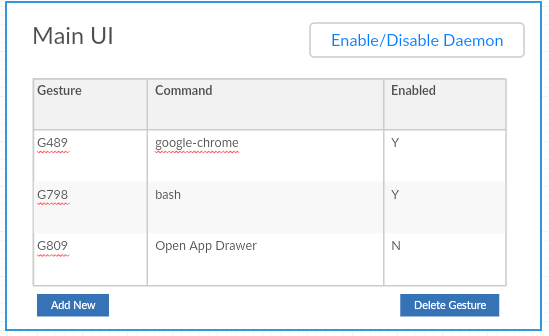
\includegraphics[scale=0.8]{mainui.png}
    \\
    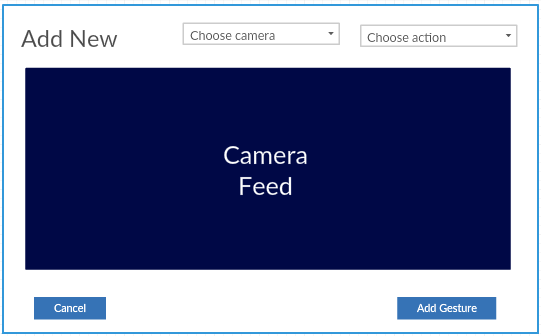
\includegraphics[scale=0.8]{addnewui.png}
\end{center}


\subsection{Hardware Interfaces}
The hardware required for the application is the webcam. The images are then handled by our application and the webcam too is managed by our deamon running in the background.

\subsection{Software Interfaces}
The daemon must interface with the camera driver and the operating system to be able to control the GUI based on input gestures.

\subsection{Communications Interfaces}
The application will need internet connection to send bug reports in case of a crash or malfunction. Bug reports will be sent in the form of HTTP requests to a remote webserver.


\newpage
\section{Hardware and Software Requirements}
\subsection{Hardware Requirements}
\begin{itemize}
    \item A computer with at least 2GHz processor, 1GB RAM and USB ports.
    \item A USB camera.
\end{itemize}

\subsection{Software Requirements}
\begin{itemize}
    \item Linux operating system.
    \\
    \\The linux operating system was chosen due to the fact that it is easy to build software due to wide range of libraries and easy access to them and the compilers. Whereas in a OS like windows a special IDE like Visual Studio and proprietary libraries would be required to build software.
    \item C++ compliler eg:- gcc
    \\
    \\C++ is a general-purpose programming language. It has imperative, object-oriented and generic programming features, while also providing facilities for low-level memory manipulation.

    It was designed with a bias toward system programming and embedded, resource-constrained and large systems, with performance, efficiency and flexibility of use as its design highlights. C++ has also been found useful in many other contexts, with key strengths being software infrastructure and resource-constrained applications, including desktop applications, servers (e.g. e-commerce, Web search or SQL servers), and performance-critical applications (e.g. telephone switches or space probes). C++ is a compiled language, with implementations of it available on many platforms.
    \\
    \\Some of the interesting features of C++ are:
    \begin{itemize}
        \item \textbf{Object-oriented}: C++ is an object-oriented programming language. This means that the focus is on “objects” and manipulations around these objects. Information about how these manipulations work is abstracted out from the consumer of the object.
        \item \textbf{Rich library support}: Through C++ Standard Template Library (STL) many functions are available that help in quickly writing code. For instance, there are standard libraries for various containers like sets, maps, hash tables, etc.
        \item \textbf{Speed}: C++ is the preferred choice when latency is a critical metric. The compilation, as well as the execution time of a C++ program, is much faster than most other general purpose programming languages.
        \item \textbf{Compiled}: A C++ code has to be first compiled into low-level code and then executed, unlike interpreted programming languages where no compilation is needed.
        \item \textbf{Pointer Support}: C++ also supports pointers which are widely used in programming and are often not available in several programming languages.
    \end{itemize}
    \item OpenCV C++ library
    \\
    \\OpenCV (Open source computer vision) is a library of programming functions mainly aimed at real-time computer vision. OpenCV is written in C++ and its primary interface is in C++. All of the new developments and algorithms in OpenCV are now developed in the C++ interface. 
    \\
    \\OpenCV has a modular structure, which means that the package includes several shared or static libraries. The following modules are available:
    \begin{itemize}
        \item \textbf{Core functionality (core)} - a compact module defining basic data structures, including the dense multi-dimensional array Mat and basic functions used by all other modules.
        \item \textbf{Image Processing (imgproc)} - an image processing module that includes linear and non-linear image filtering, geometrical image transformations (resize, affine and perspective warping, generic table-based remapping), color space conversion, histograms, and so on.
        \item \textbf{Video Analysis (video)} - a video analysis module that includes motion estimation, background subtraction, and object tracking algorithms.
        \item \textbf{Camera Calibration and 3D Reconstruction (calib3d)} - basic multiple-view geometry algorithms, single and stereo camera calibration, object pose estimation, stereo correspondence algorithms, and elements of 3D reconstruction.
        \item \textbf{2D Features Framework (features2d)} - salient feature detectors, descriptors, and descriptor matchers.
        \item \textbf{Object Detection (objdetect)} - detection of objects and instances of the predefined classes (for example, faces, eyes, mugs, people, cars, and so on).
        \item \textbf{High-level GUI (highgui)} - an easy-to-use interface to simple UI capabilities.
        \item \textbf{Video I/O (videoio)} - an easy-to-use interface to video capturing and video codecs.
    \end{itemize}


    OpenCV has functions available for background subtraction. Several algorithms were introduced for this purpose. OpenCV has implemented three such algorithms which are very easy to use like BackgroundSubtractorMOG, BackgroundSubtractorMOG2 and BackgroundSubtractorGMG.
    
    OpenCV also has various feature extractors that can be used for detect the fingers of the user like CvFeatureEvaluator, CvFeatureParams, CvHaarEvaluator and CvHaarFeatureParams.
    \item GTK+ Library for C++
    \\
    \\GTK+, or the GIMP Toolkit, is a multi-platform toolkit for creating graphical user interfaces. Offering a complete set of widgets, GTK+ is suitable for projects ranging from small one-off tools to complete application suites.
    \\
    \\The GTK+ Library is needed to build an interactive GUI where users can configure the Gesture Control System. Functions to create windows and other GUI elements such as buttons, lists, pop-ups, drop-downs, frames to display video, etc are available in the library. The library also allows to bind functions to events in the GUI such as clicks, key-presses and so on.
    \\
    \\Features of GTK+:
    \begin{itemize}
        \item \textbf{Stability}: GTK+ has been developed for over a decade to be able to deliver the enticing features and superb performance that it brings to your application development. GTK+ is supported by a large community of developers and has core maintainers from companies such as Red Hat, Novell, Lanedo, Codethink, Endless Mobile and Intel.
        \item \textbf{Interfaces}: GTK+ has a comprehensive collection of core widgets and interfaces for use in your application.
        \item \textbf{Cross Platform}: Originally GTK+ was developed for the X Window System but it has grown over the years to include backend support for other well known windowing systems. Today you can use GTK+ on Windows, Mac OS X and Linux.
        \item \textbf{Accommodating}: GTK+ caters for a number features that today's developers are looking for in a toolkit including Native look and feel, Theme support, Thread safety and Object oriented approach.
        \item \textbf{Foundation}: GTK+ is built on top of GLib. GLib provides the fundamental algorithmic language constructs commonly duplicated in applications.
    \end{itemize}
\end{itemize}

\section{Functional Requirements}
\subsection{Start/Stop the Hand Gesture Daemon}
A toggle button that starts and stops the deamon which tracks hand gestures.
\begin{center}
    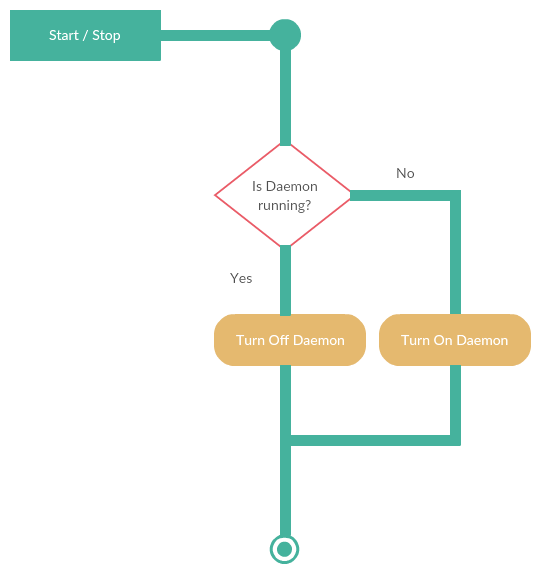
\includegraphics[scale=0.5]{start.png}
\end{center}
Input: Toggle button
\\Process: Will stop/start the daemon in the background
\\Output: The daemon shall be stopped/started.

\subsection{Add new gestures}
The user should be able to add new gestures by recording the hand movement and mapping the GUI feature to the current Hand gesture.
\begin{center}
    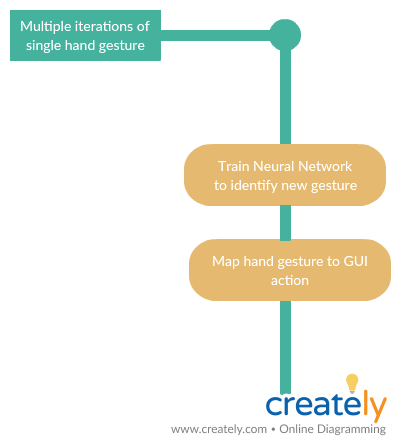
\includegraphics[scale=0.5]{add.png}
\end{center}
Input: Multiple Iterations of a gesture via Camera; Action to carry out
\\Process: The software will train the Neural Network to identify the new hand gesture and map the hand gesture to the Command given as input
\\Output: A new mapping from the hand gesture to the command will be added

\subsection{Remove gestures}
The user can remove the existing gestures
\begin{center}
    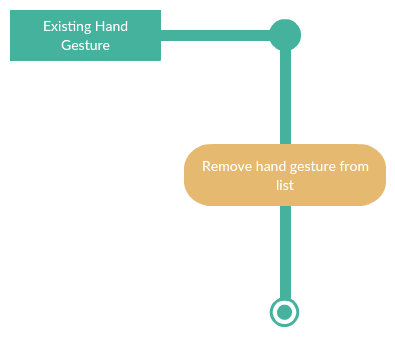
\includegraphics[scale=0.5]{remove.png}
\end{center}
Input: A hand gesture
\\Process: The software will remove the mapping of the input hand gesture from the list of hand gestures
\\Output: The hand gesture is removed
 
\subsection{Modify Gestures}
\begin{center}
    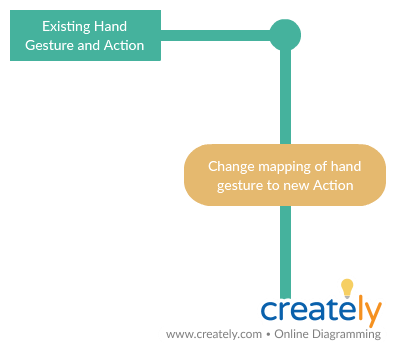
\includegraphics[scale=0.5]{modify.png}
\end{center}
Input: Existing hand gesture; Action to execute
\\Process: The software will change the mapping of the input hand gesture to the input Action
\\Output: The hand gesture is modified

 \subsection{Choose webcam}
For systems with multiple webcams connected the user must be able to choose which webcam the application must use.
\begin{center}
    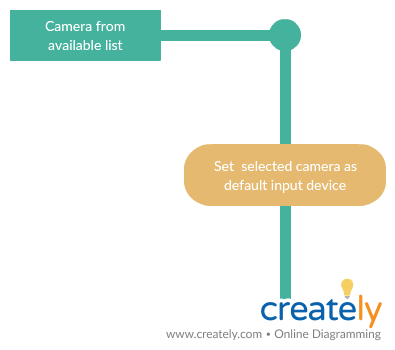
\includegraphics[scale=0.5]{camera.png}
\end{center}
Input: A camera detected by the daemon
\\Process: The software will set the selected camera as the default input for images
\\Output: The daemon will now watch for gestures through the selected camera when activated

\section{Non-functional Requirements}    
\subsection{Performance Requirements}
The product must be fast enough to recognize and execute the hand gesture such that the action becomes fluid. The product must be responsive all the time and multiple hand gestures shown rapidly must be processed effectively.

\subsection{Safety Requirements}
No other application or user should access the camera feed.

\subsection{Security Requirements}
The camera feed must not be stored in the system. No one should be able to tap into the camera feed or be able to extract information from the camera.

\subsection{Software Quality Attributes}

Our product must be adaptable to all lighting conditions, poor webcams, and poor system capabilities. The product will be easy to maintain and review for other people. The  product will run on newer updates of the operating system without any glitches.

\section{Other Requirements}
The product can be reused by other developers to create and maintain their own products. The GUI of the application must work with all languages so that people from all backgrounds can work seamlessly. 




\chapter{System Design}
\section{System Architecture}
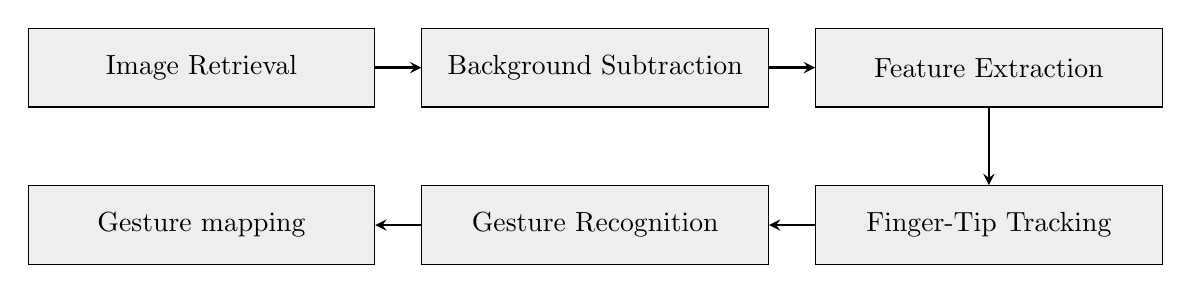
\begin{tikzpicture}[node distance=5cm]
    \node (proc1) [process] {Image Retrieval};
    \node (proc2) [process, right of = proc1] {Background Subtraction};
    \node (proc3) [process, right of = proc2] {Feature Extraction};
    \node (proc4) [process, below of = proc3, yshift = 3cm] {Finger-Tip Tracking};
    \node (proc5) [process, left of = proc4] {Gesture Recognition};
    \node (proc6) [process, left of = proc5] {Gesture mapping};
    \draw [arrow] (proc1) -- (proc2);
    \draw [arrow] (proc2) -- (proc3);
    \draw [arrow] (proc3) -- (proc4);
    \draw [arrow] (proc4) -- (proc5);
    \draw [arrow] (proc5) -- (proc6);
\end{tikzpicture}

\section{Use case diagram}
\begin{center}
    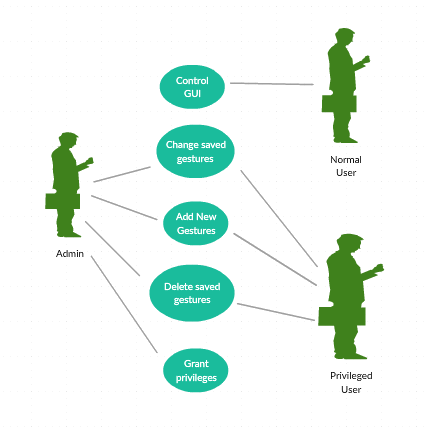
\includegraphics{usecase.png}
\end{center}
\section{Class diagram}
\begin{center}
    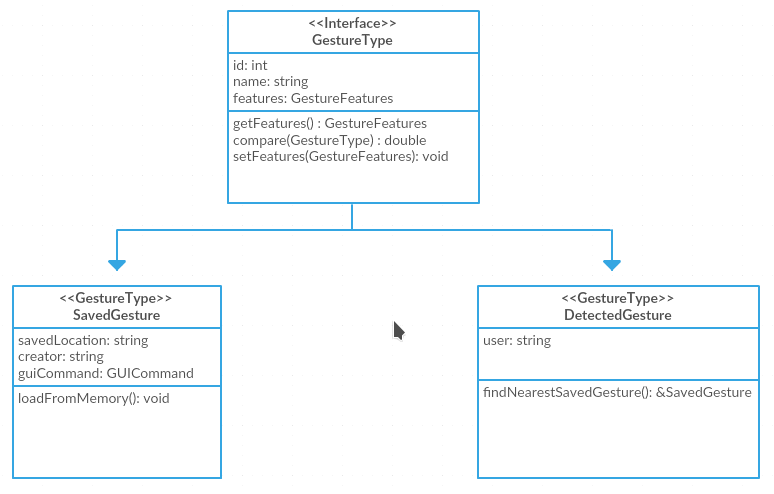
\includegraphics[width=14cm]{classdiagram.png}
    \vspace{10cm}
    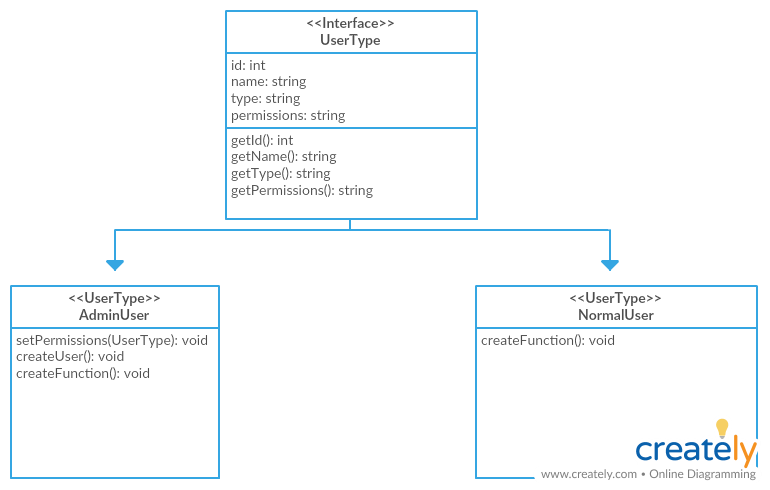
\includegraphics[width=14cm]{UserClass.png}
\end{center}
\section{Activity diagram}
\begin{center}
    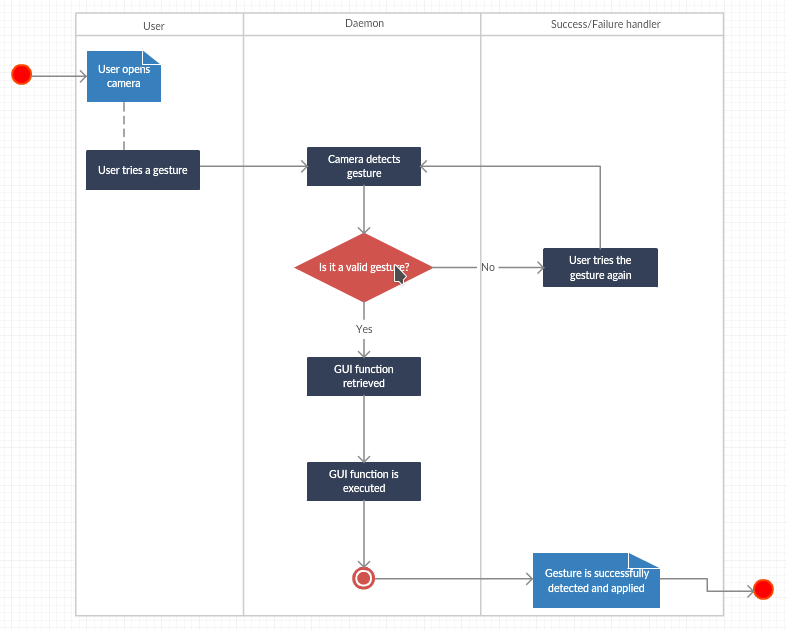
\includegraphics[scale=0.8]{activitydiagram.png}
\end{center}

\section{Input Design}
    In the system, the hand gesture is captured by the web cam in multiple frames. After the gesture Is
    carried out, it is recognized and the corresponding GUI command is carried out.

% \section{Database Design}
\section{Libraries and Packages Used}


\section{Module Description}

\subsection{Module 1 - Image Retrieval}
The first step in this system is to retrieve the contiguous camera image frames. The user shows the hand-gesture 
and it is retrieved via the webcam. The images are captured at short intervals to accommodate multi-frame fluid hand-gestures.
\\
The camera feed is retrieved from the user's webcam using the CaptureFromCAM function provided by OpenCV.
\\
The function reads an image from the specified buffer in the memory. If the buffer is too short or contains invalid data, the empty matrix/image is returned.
\subsection{Module 2 - Background Subtraction}
The captured image from the camera needs to undergo background subtraction in order to recognize the gesture correctly. 
The different elements in the background has to be discarded and only the shape of the hand is retained. 
\\
The captured image from the camera needs to undergo background subtraction in order to recognize the gesture correctly. The different elements in the background has to be discarded and only the shape of the hand is retained.  
We convert the BGR image to HSV image using cv::cvtColor() function
We use cv::inRange function to get the Hue,Saturation and Value as ranges of the saved HSV val
\subsection{Module 3 - Feature Extraction}
The next step is to find the fingertip locations in the recorded image from the background subtracted image.
To recognize the fingertips we use the Convex Hull algorithm. 
\\
The locations of the fingertips on the screen are detected by finding the Convex hull of the 
hand and marking the peaks. This process is done in realtime and the extracted location changes
 with every frame. 
 
 The function find the convex hull of a 2D point set using the Sklansky’s algorithm
 that has O(N logN) complexity in the current implementation. The algorithm consisted of two parts. 
 Part 1 was intended to take a simple polygon and return a maximal polygon (monotonic in both the 
 horizontal and vertical directions). Part 2 was Sklansky's original algorithm, which
 was guaranteed to work on the output of part 1, since maximal polygons are weakly externally visible,
 and it is proven that Sklansky's original algorithm works for such polygons.

\subsection{Module 4 - Finger-Tip Tracking}
We compute the centroid of the convex hull of each finger. The formula of convex hull is as follows.
\begin{center}
    
\begin{figure}[H]
    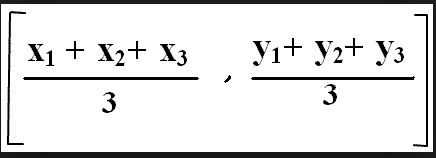
\includegraphics[width=4cm]{centroid.png}
\end{figure}
\end{center}


\subsection{Module 5 - Gesture Recognition}
After extracting the finger tip information, we need to track the finger tips over multiple frames. 
A brute force matching method has been used to detect swipes (up, down, right left). The FingertipDetectionModule
module has been implemented for the same purpose.

\subsection{Module 6 - Gesture Mapping}

Once the correct gesture has been identified, 
the corresponding class object is accessed to procure the GUI function that has been saved 
for that particular gesture. The function is first executed, and then the daemon starts listening 
for the next gesture.

\chapter{Data Flow Diagram}

\section{Level 0}
\resizebox{\columnwidth}{!}{
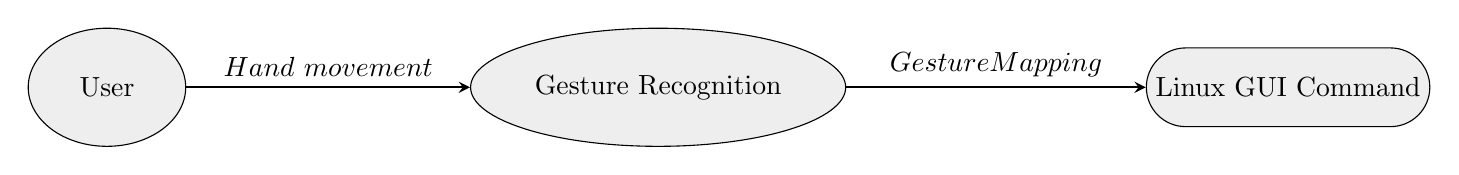
\begin{tikzpicture}[node distance=7cm]
    \node (proc1) [oval2]{User};
    \node (proc2) [oval2, minimum width=10mm,right of = proc1]{Gesture Recognition};
    \node (proc3) [process1,minimum size=10 mm, right of = proc2,xshift= 10 mm]{Linux GUI Command};

    \draw[arrow] (proc1)--(proc2) node[midway,above,rotate=0] {$Hand\ movement$};
    \draw[arrow] (proc2)--(proc3) node[midway,above,rotate=0] {$Gesture Mapping$};
%    \draw [black] ([yshift=0.2cm]proc3.west)--([yshift=0.2cm]proc3.east);

\end{tikzpicture}}
\\
\section{Level 1}
\resizebox{\columnwidth}{!}{
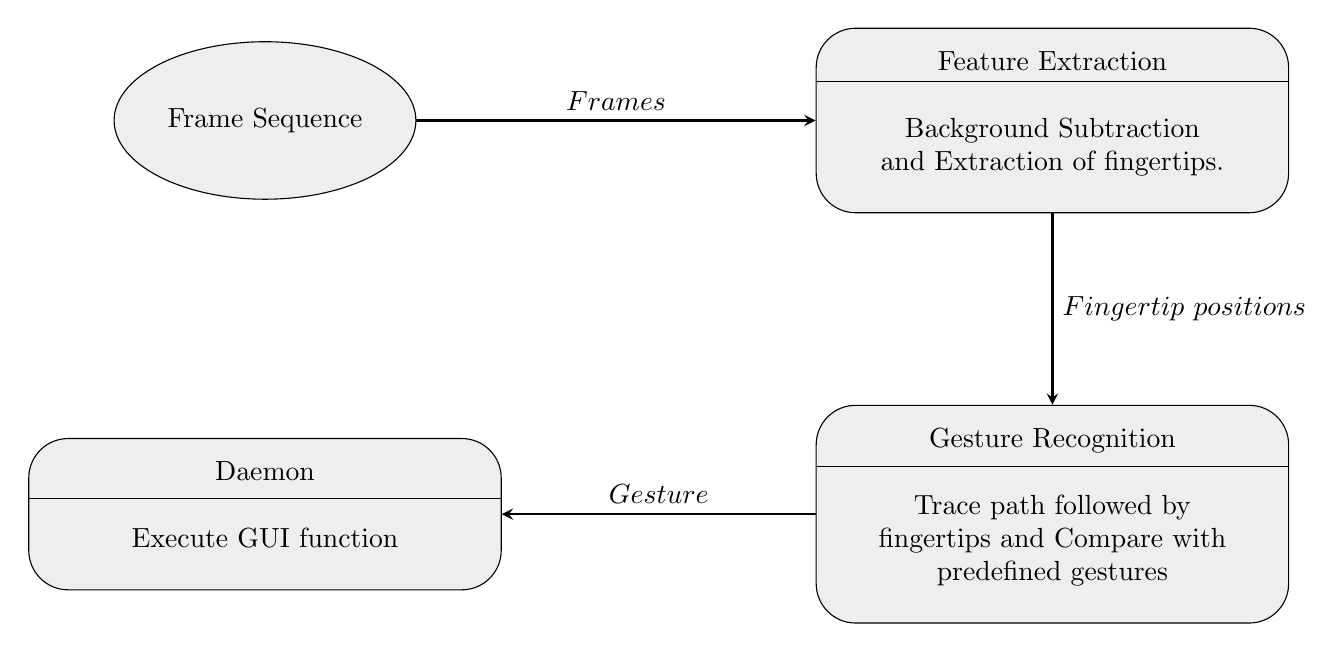
\begin{tikzpicture}[node distance=2cm]
    \node (proc1) [oval]{Frame Sequence};
    \node (proc2) [process1, right of = proc1, xshift=8 cm]{\\Feature Extraction\\\\
    Background Subtraction\\
    and Extraction of fingertips.\\};
    \node (proc3) [process1, below of = proc2, yshift=-3cm]{\\Gesture Recognition\\\\
    Trace path followed by\\
    fingertips and Compare with\\
    predefined gestures\\};
    \node (proc4) [process1, left of = proc3, xshift=-8cm]{\\Daemon\\\\Execute GUI function\\};
    \draw[arrow] (proc1)--(proc2) node[midway,above,rotate=0] {$Frames$};
    \draw[arrow] (proc2)--(proc3) node[midway,right,rotate=0]{$Fingertip\ positions$};
    \draw[arrow] (proc3)--(proc4) node[midway,above,rotate=0] {$Gesture$};
    \draw [black] ([yshift=0.5cm]proc2.west)--([yshift=0.5cm]proc2.east);
    \draw [black] ([yshift=0.6cm]proc3.west)--([yshift=0.6cm]proc3.east);
    \draw [black] ([yshift=0.2cm]proc4.west)--([yshift=0.2cm]proc4.east);
\end{tikzpicture}}

\section{Level 2}
\resizebox{\columnwidth}{!}{
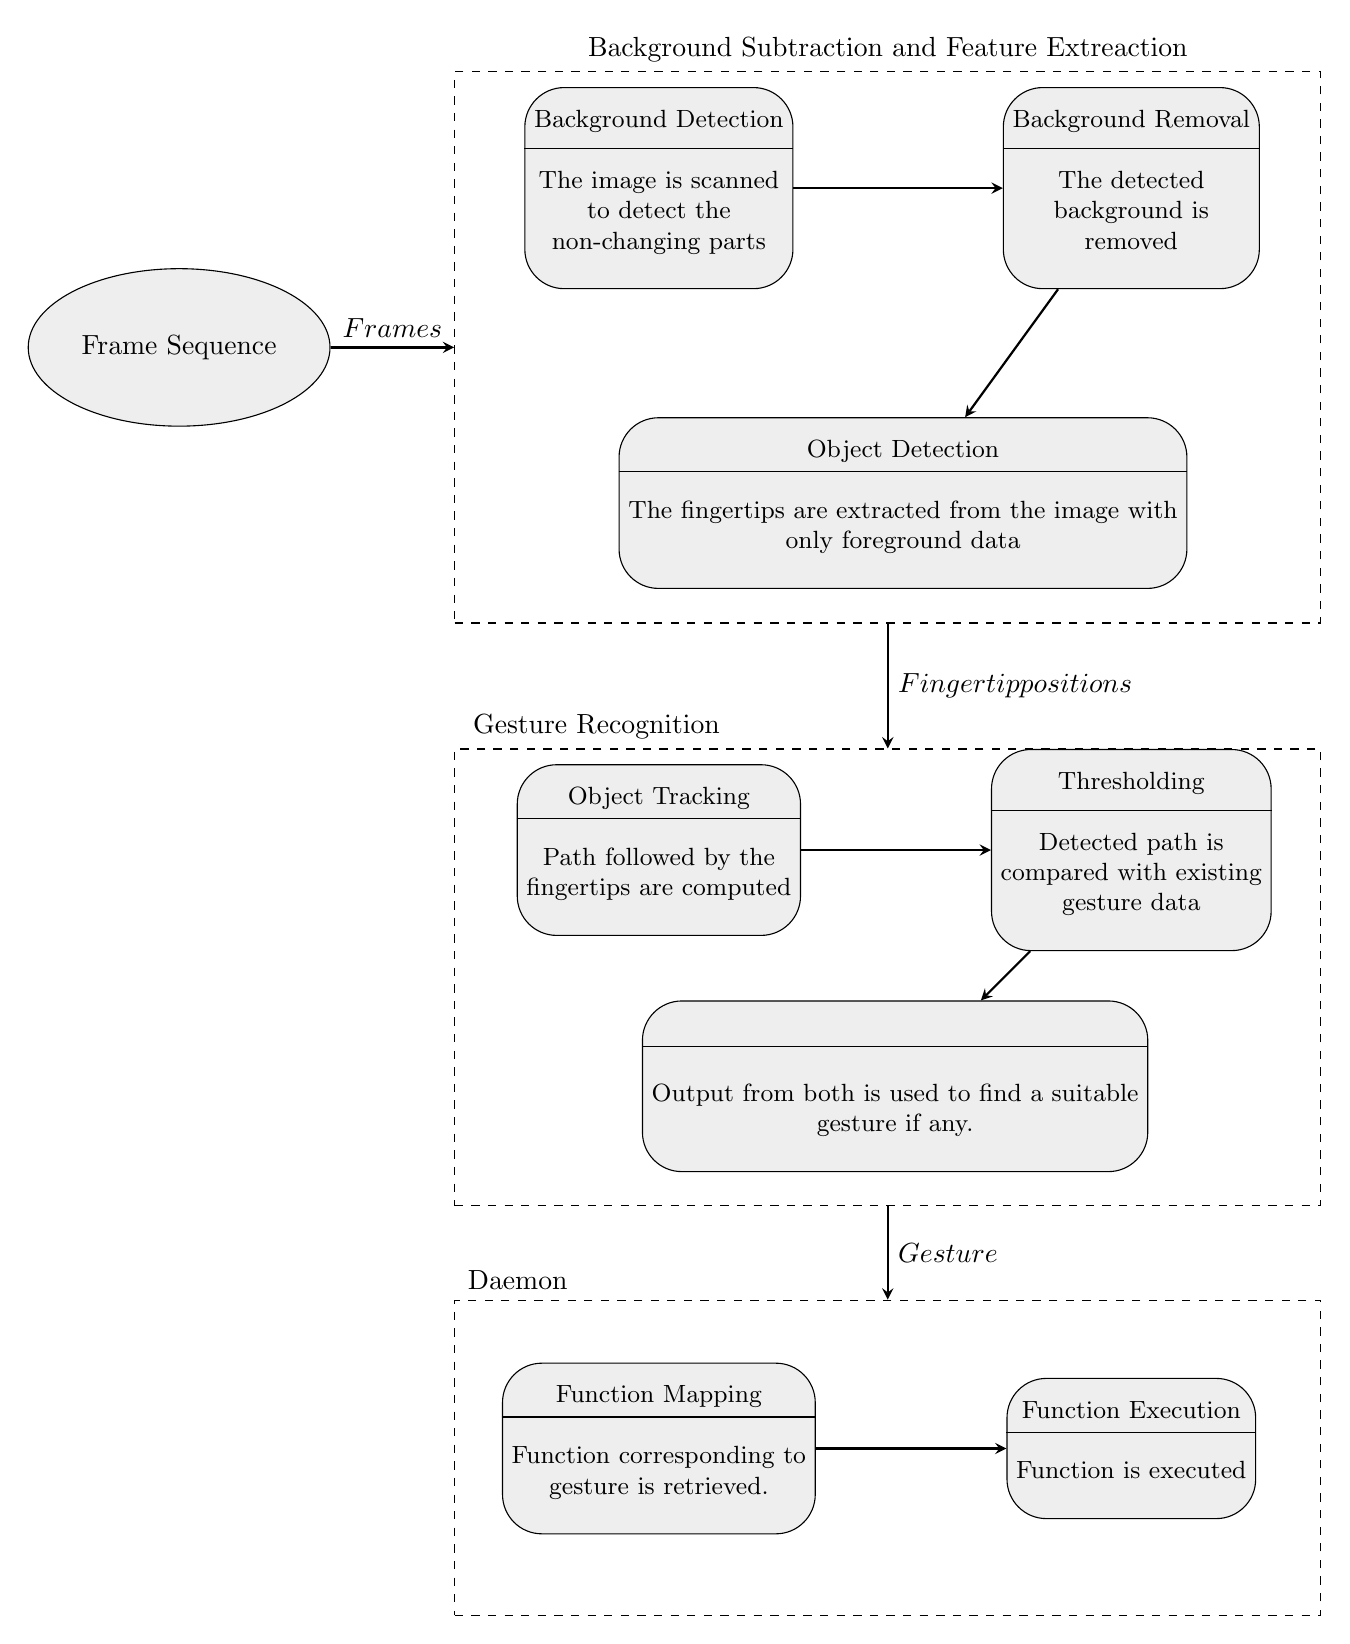
\begin{tikzpicture}[node distance=0cm]
    \node (proc1) [oval]{Frame Sequence};

    \node (over1) [overlay, label=above:Background Subtraction and Feature Extreaction, minimum width = 11cm, minimum height = 7cm, right of = proc1, xshift=9cm]{};

    \node (proc2) [process2, below=of over1.north west, xshift=2.6cm, yshift=-0.2cm]{\\Background Detection\\\\
    The image is scanned\\
    to detect the\\
    non-changing parts\\};


    \node (proc3) [process2, right of = proc2, xshift=6cm]{\\Background Removal\\\\
    The detected\\
    background is\\
    removed\\};

    \node (proc4) [process2, left of = proc3, xshift=-2.9cm, yshift=-4cm]{\\Object Detection\\\\
    The fingertips are extracted from the image with\\
    only foreground data\\};

    \draw [arrow] (proc1)--(over1) node[midway,above,rotate=0] {$Frames$};
    \draw [black] ([yshift=0.5cm]proc2.west)--([yshift=0.5cm]proc2.east);
    \draw [black] ([yshift=0.5cm]proc3.west)--([yshift=0.5cm]proc3.east);
    \draw [black] ([yshift=0.4cm]proc4.west)--([yshift=0.4cm]proc4.east);
    \draw [arrow] (proc2)--(proc3) node[midway, above]{$$};
    \draw [arrow] (proc3)--(proc4) node[midway, above]{$$};
    \node (over2) [overlay, label={[xshift=-3.7cm]Gesture Recognition}, minimum width = 11cm, minimum height = 5.8cm, right of = over1, yshift=-8cm]{};

    \node (proc5) [process2, below=of over2.north west, xshift=2.6cm, yshift=-0.2cm]{\\Object Tracking\\\\
    Path followed by the\\
    fingertips are computed\\};

    \node (proc6) [process2, right of = proc5, xshift=6cm]{\\Thresholding\\\\
    Detected path is\\
    compared with existing\\
    gesture data\\};

    \node (proc7) [process2, left of = proc6, xshift=-3cm, yshift=-3cm]{\\\\\\
    Output from both is used to find a suitable\\
    gesture if any.\\};
    \draw [arrow] (over1)--(over2) node[midway, right]{$Fingertip positions$};
    \draw [black] ([yshift=0.4cm]proc5.west)--([yshift=0.4cm]proc5.east);
    \draw [black] ([yshift=0.5cm]proc6.west)--([yshift=0.5cm]proc6.east);
    \draw [black] ([yshift=0.5cm]proc7.west)--([yshift=0.5cm]proc7.east);
    \draw [arrow] (proc5)--(proc6) node[midway, below]{$$};
    \draw [arrow] (proc6)--(proc7) node[midway, below]{$$};

    \node (over3) [overlay, label={[xshift=-4.7cm]Daemon}, minimum width = 11cm, minimum height = 4cm, right of = over2, yshift=-6.1cm]{};

    \node (proc8) [process2, below=of over3.north west, xshift=2.6cm, yshift=-0.8cm]{\\Function Mapping\\\\
    Function corresponding to\\
    gesture is retrieved.\\};

    \node (proc9) [process2, right of = proc8, xshift=6cm]{\\Function Execution\\\\
    Function is executed\\};
    \draw [arrow] (proc8)--(proc9) node[midway, below]{$$};

    \draw [arrow] (over2)--(over3) node[midway, right]{$Gesture$};

    \draw [black] ([yshift=0.4cm]proc8.west)--([yshift=0.4cm]proc8.east);
    \draw [black] ([yshift=0.2cm]proc9.west)--([yshift=0.2cm]proc9.east);

\end{tikzpicture}}

\chapter{Implementation}
\section{Algorithms}
\subsection{Overall algorithm}
\begin{itemize}
    \item Input: A set of contiguous image frames
    \item Output: The mapped GUI function
    \item Method:
    \begin{enumerate}
        \item Calculate the foreground using background subtraction algorithm.
        \item Detect the fingertips using the Convex Hull algorithm.
        \item Track the finger gesture using Brute Force Matching.
        \item Save the above tracked graph to a DetectedGesture object.
        \item Find the closest SavedGesture object and execute the GUI function.
    \end{enumerate}
\end{itemize}
\subsection{Background subtraction}
\begin{enumerate}
    \item Purpose: To find the Region of Interest by subtracting the background from the image frame.
    \item Input: Image frames with foreground and background.
    \item Output: Image frames with only foreground. 
    \item Method:
    \begin{itemize}
        \item Model each background pixel by a mixture of K Gaussian distributions (K = 3 to 5)
        \item Calculate the weights of the mixture which represent the time proportions that those colours stay in the scene.
        \item Remove the colours are which stay longer and more static.
    \end{itemize}
\end{enumerate}
\subsection{Convex Hull}
\begin{itemize}
    \item Purpose: To find the positions of the fingertips in the image frame.
    \item Input: Image frames with background subtracted.
    \item Output: List of Convex Hull peaks
    \item Method:
    \begin{enumerate}
        \item Threshold the image, and retrieve the points in the plane. Let's say there are P points.
        \item Initialize p as leftmost point.
        \item Do following while we don’t come back to the first (or leftmost) point.
        \begin{enumerate}
            \item The next point q is the point such that the triplet (p, q, r) is counterclockwise for any other point r.
            \item next[p] = q (Store q as next of p in the output convex hull).
            \item p = q (Set p as q for next iteration).
        \end{enumerate}
    \end{enumerate}
\end{itemize}
\subsection{Brute Force Matching}
\begin{itemize}
    \item Purpose: To map the positions of the fingertips in the multiple frames to one fluid motion, in the form of lines/curves in a 2D plane.
    \item Input: The points pertaining to a gesture (with minimal jitter)
    \item Output: A value representing the swipe direction and distance between points.
    \item Method:
    \begin{enumerate}
        \item For a given keypoint K1 from the first set, take the next keypoint in the set and calculate the distance.
        \item Choose the initial location of the two-dimensional mean shift search window.
        \item Calculate the colour probability distribution in the 2D region centred on the search window location in an area slightly larger than the mean shift window size.
        \item Perform the search of the maximum density probability using the mean shift parameter for convergence or for setting the number of iterations. Store the zero moment (area or size) and middle position.
        \item For the next image frame, place the search window in the middle position fixed in step 4, and set the window size in conformity to the last moment. Go to step 3. 
    \end{enumerate}
\end{itemize}
\subsection{Brute Force Matching}
\begin{itemize}
    \item Purpose: To match the DetectedGesture to a SavedGesture, and execute the corresponding GUI function.
    \item Input: The feature objects encoded in the SavedFeature and DetectedFeature objects.
    \item Output: A quantity representing the closeness of the two gestures.
    \item Method:
    \begin{enumerate}
        \item For a given keypoint K1 from the first set, take every keypoint in the second set and calculate the distance.
        \item Distance formula used is Euclidean distance. The sum of the distances on each dimension is finally used to calculate the returned quantity.
        \item Distance formula used is Euclidean distance. The sum of the distances on
        each dimension is finally used to calculate the returned quantity.
        \item If the distance is lesser than a threshold, then flush the buffer because the gesture is too slow.
        \item Keep Jitter Tolerance to a useful value (like 5) and flush the buffer if the number of jitter values exceeds 5.
        \item If the buffer length reaches a value, the distanceAndDirectionFrom function helps to get the type of swipe.
    \end{enumerate}
\end{itemize}
\section{Development Tools}
\subsection{Sublime Text}
Sublime Text is a proprietary cross-platform source code editor with a Python application program-
ming interface (API). It natively supports many programming languages and markup languages,
and functions can be added by users with plugins, typically community-built and maintained under
free-software licenses.
Some of the features of Sublime Text are
\begin{itemize}
\item ”Goto Anything,”quick navigation to files, symbols, or lines
\item ”Command palette” uses adaptive matching for quick keyboard invocation of arbitrary com-
mands
\item Simultaneous editing: simultaneously make the same interactive changes to multiple selected
areas

\item Project-specific preferences

\item Cross platform (Windows, macOS, and Linux)

\end{itemize}

\chapter{Testing}
Software testing is an investigation conducted to provide stakeholders with information about
the quality of the product or service under test. Software testing can also provide an objective,
independent view of the software to allow the business to appreciate and understand the risks of
software implementation. Test techniques include the process of executing a program or application
with the intent of finding software bugs, and to verify that the software product is fit for use.
Software testing involves the execution of a software component or system component to evaluate
one or more properties of interest. In general, these properties indicate the extent to which the
component or system under test
\begin{itemize}
    \item Meets the requirements that guided its design and development,
    \item Responds correctly to all kinds of inputs
    \item Performs its functions within an acceptable time
\item Is sufficiently usable
\item Can be installed and run in its intended environments, and
\item Achieves the general result its stakeholders desire.
\end{itemize}
\section{Testing Methodologies}
Software testing methodology is for making sure that software products/systems developed have
been successfully tested to meet their specified requirements and can successfully operate in all the
anticipated environments with required usability and security.
Software testing methods are traditionally divided into white and black-box testing. These two
approaches are used to describe the point of view that a test engineer takes when designing test
cases.
White-box testing by seeing the source code tests internal structures or workings of a program, as
opposed to the functionality exposed to the end-user. In white-box testing an internal perspective
of the system, as well as programming skills, are used to design test cases. The tester chooses in-
puts to exercise paths through the code and determine the appropriate outputs. This is analogous
to testing nodes in a circuit. While white-box testing can be applied at the unit, integration and system levels of the software testing process, it is usually done at the unit level.
Black-box testing treats the software as a black-box , examining functionality without any knowl-
edge of internal implementation, without seeing the source code. The testers are only aware of
what the software is supposed to do, not how it does it. Here the black-box testing is used for the
system. The testing methods applied were:

\begin{itemize}
    \item Unit Testing \\
Unit testing is a software development process in which the smallest testable parts of an
application, called units, are individually and independently scrutinized for proper operation.
    \item Integration Testing \\
    Integration testing is the phase in software testing in which individual software modules are
    combined and tested as a group. It occurs after unit testing.
    \item System Testing \\
    System testing of software or hardware is testing conducted on a complete, integrated system
    to evaluate the system’s compliance with its specified requirements. System testing falls
    within the scope of black-box testing, and as such, should require no knowledge of the inner
    design of the code or logic.
\end{itemize}
\section{Unit Testing}
In the unit testing phase, the Background Subtraction Module, Feature Extraction, Finger-tip Tracking, Gesture Recognition
and Gesture mapping were separately tested.

\subsection{Background Subtraction Module}

The images from the camera feed is provided to the Background Subtraction
module in RGB colour space. The output images were in HSV filtered with Colour Ranges as expected.

\begin{figure}[h]
    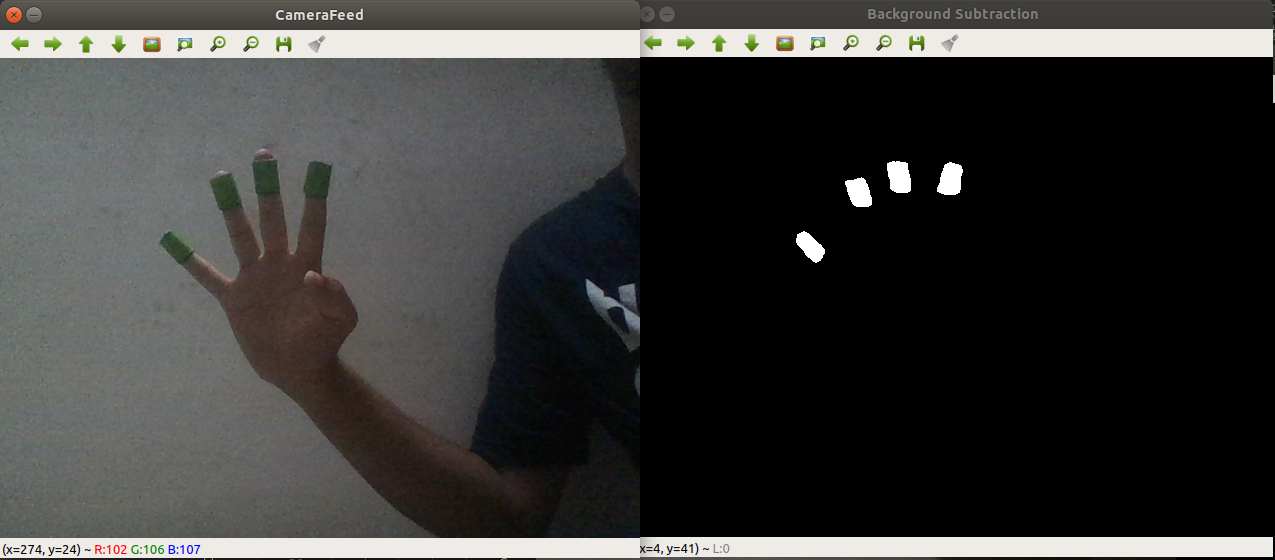
\includegraphics[width=15cm]{backgroundtesting.png}
    \caption{Background Subtraction Module}
\end{figure}

\subsection{Feature Extraction}

The output from the background subtraction module is fed into the feature Extraction
module. This module computes the convex hull and finds the separate shapes and finds the centroids of 
each hull.

\begin{figure}[h]
    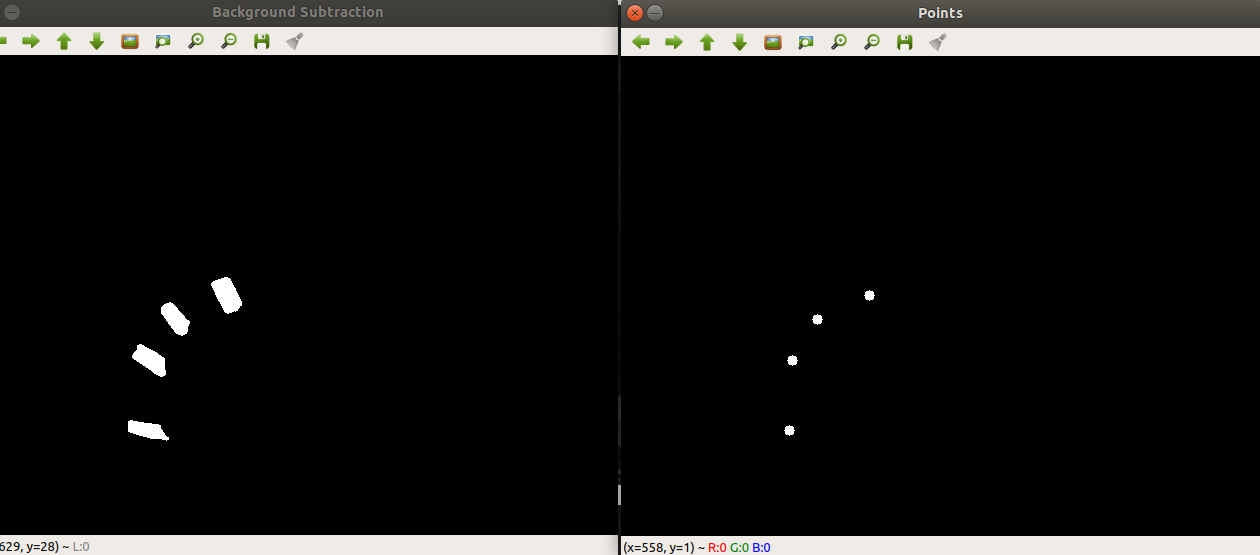
\includegraphics[width=15cm]{featuretest.png}
    
    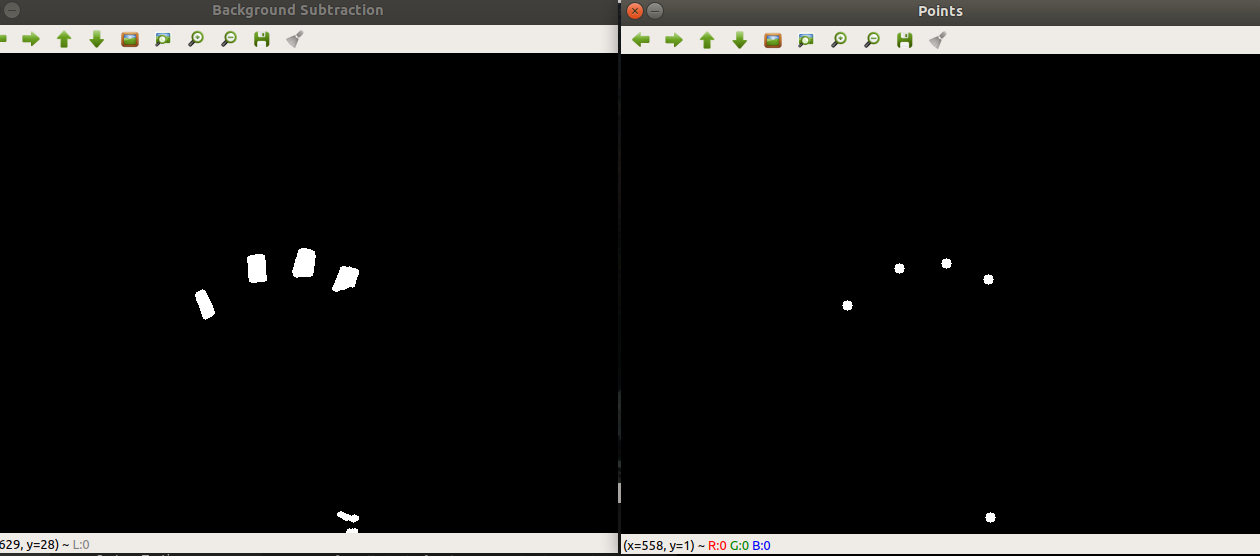
\includegraphics[width=15cm]{featuretest2.png}
    \caption{Feature Extraction Module}
\end{figure}

\subsection{FingerTip Tracking and Gesture Recognition}

The Finger tip tracking module tracks the centroids movement over multiple frames and the Gesture Recognition Module recognizes the gesture.

\begin{figure}[H]
    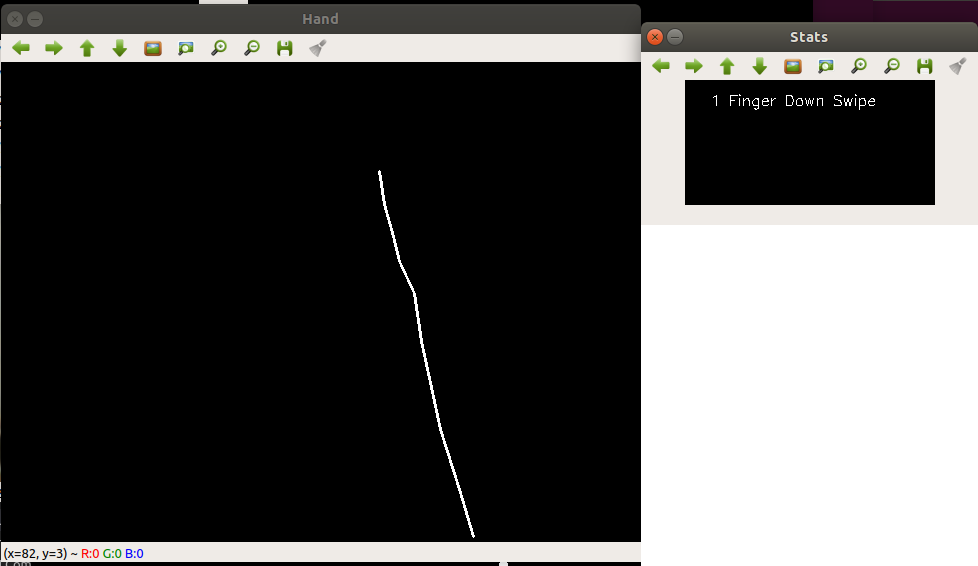
\includegraphics[width=15cm]{gesture.png}
    
    \caption{Finger Tip Tracking and Gesture Recognition}
\end{figure}



\section{Integration Testing}

Different modules were combined and was tested to see if the modules interact properly and produce
correct output. The Background Subtraction Module provided its output to the feature extraction module
which then finds the convex hulls. The output is passed to the finger-tip tracking module which tracks the 
direction and number of fingers. The output is successfully passed to the Gesture Recognition module which allots the gesture.
Finally the output is passed to the Gesture Map module which executes the gesture in the Linux GUI.

\section{System Testing}

After the integration testing, we do the system testing. In system testing the whole modules are
connected in order; the background subtraction module is integrated with the feature extraction module,the
feature extraction module is integrated with the fingertip tracking and also the gesture recognition
module and gesture mapping module. The whole system is inte-
grated.



\chapter{Graphical User Interface}
The graphical user interface (GUI ), is a type of user interface that allows users to interact with
electronic devices through graphical icons and visual indicators such as secondary notation, instead
of text-based user interfaces, typed command labels or text navigation. GUI's were introduced in
reaction to the perceived steep learning curve of command-line interfaces which require commands
to be typed on a computer keyboard.
Designing the visual composition and temporal behavior of a GUI is an important part of
software application programming in the area of human-computer interaction. Its goal is to enhance
the efficiency and ease of use for the underlying logical design of a stored program, a design discipline
named usability. Methods of user-centered design are used to ensure that the visual language
introduced in the design is well-tailored to the tasks.
For several decades, GUIs were controlled exclusively by a mouse and a keyboard. While these
types of input devices are sufficient for desktop computers, they do not work as well for mobile
devices, such as smart-phones and tablets. Therefore, mobile operating systems are designed to use
a touchscreen interface. Many mobile devices can now be controlled by spoken commands as well.
Because there are now many types of digital devices available, GUI's must be designed for the
appropriate type of input. For example, a desktop operating system, such as OS X, includes a
menu bar and windows with small icons that can be easily navigated using a mouse. A mobile OS,
like iOS, includes larger icons and supports touch commands like swiping and pinching to zoom in
or zoom out. Automotive interfaces are often designed to be controlled with knobs and buttons,
and TV interfaces are built to work with a remote control. Regardless of the type of input, each of
these interfaces are considered GUI's since they include graphical elements.
\section{GUI Overview}

For the proposed system, the GUI is built using the GTK library. We have components for Mapping out the 
different gestures, calibrating the system, Adding and Remove Mappings to Gestures.  

\section{Main GUI Components}


\subsection{Calibrate Detection}
    To Calibrate the colors detected which may vary from due to lighting conditions. This component allows
    the user to refine the background subtraction module by providing an image frame of the current placement of the hand which
    extracts the colours in the image frame.
    \begin{figure}[H]
    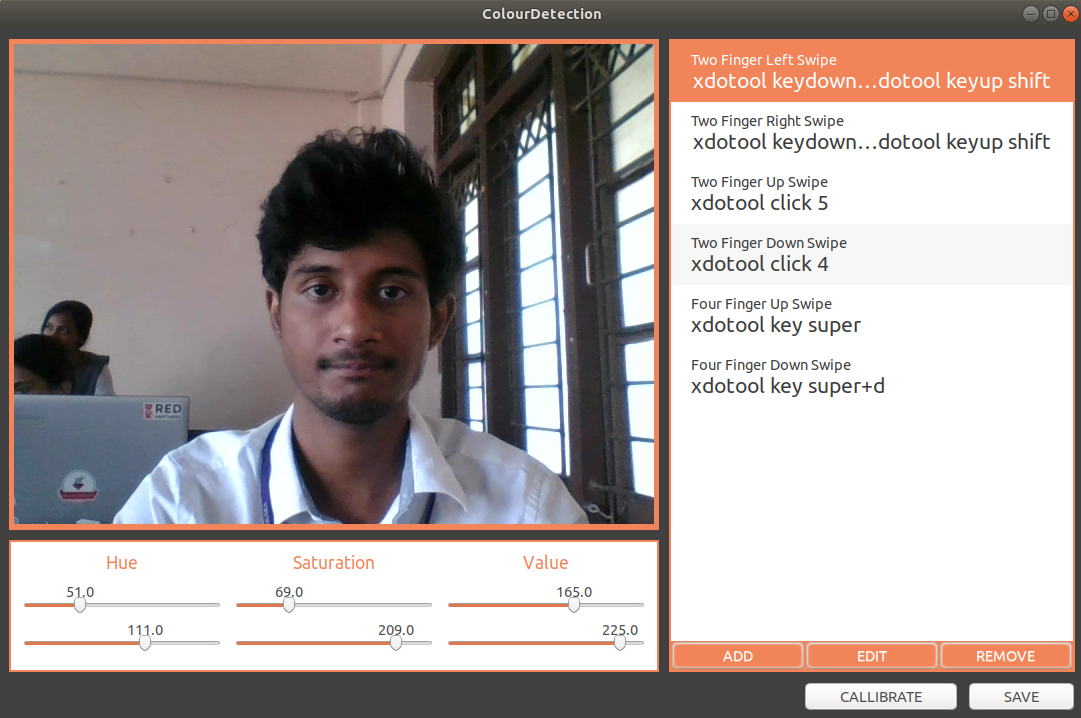
\includegraphics[width=14cm]{1.png}
    \label{Calibrate Detection}
    \caption{Calibrate Detection}
    \end{figure}
\subsection{Gesture Mapping}

    This module allows to map the gestures to Linux GUI commands. Each gesture can be mapped according to 
    the users wish. It also allows the user to remove a gesture mapping or add a new gesture mapping.
    \begin{figure}[H]
        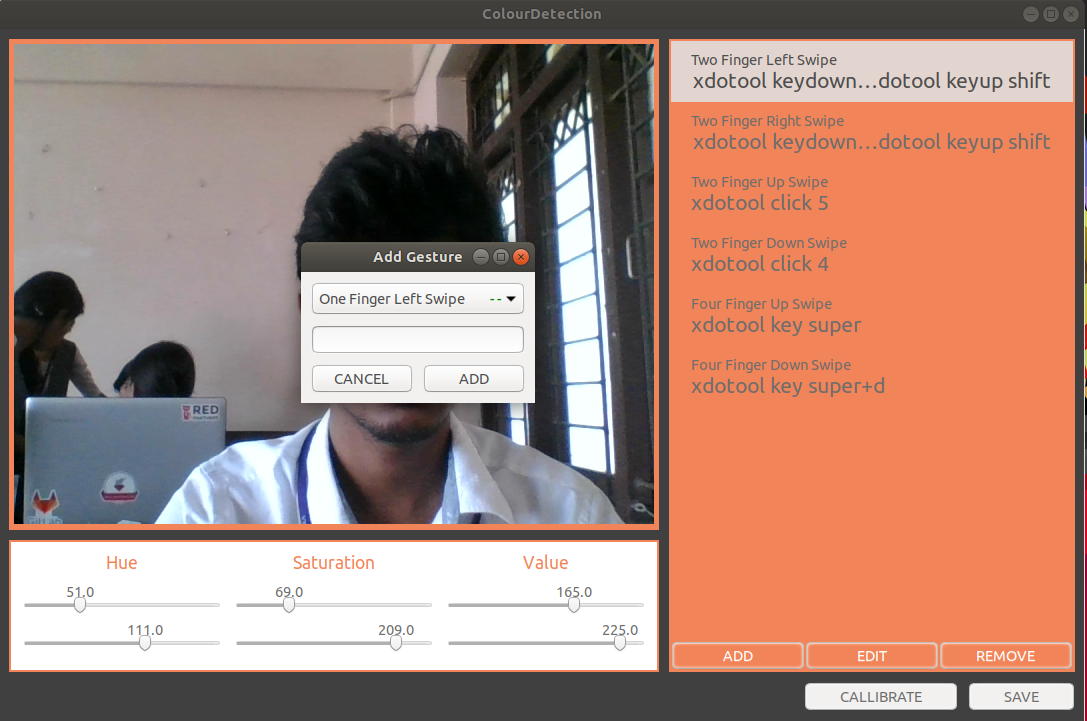
\includegraphics[width=14cm]{2.png}
        \label{Map Gesture}
        \caption{Map Gesture}
        \end{figure}

\chapter{Results}
\begin{figure}[H]
    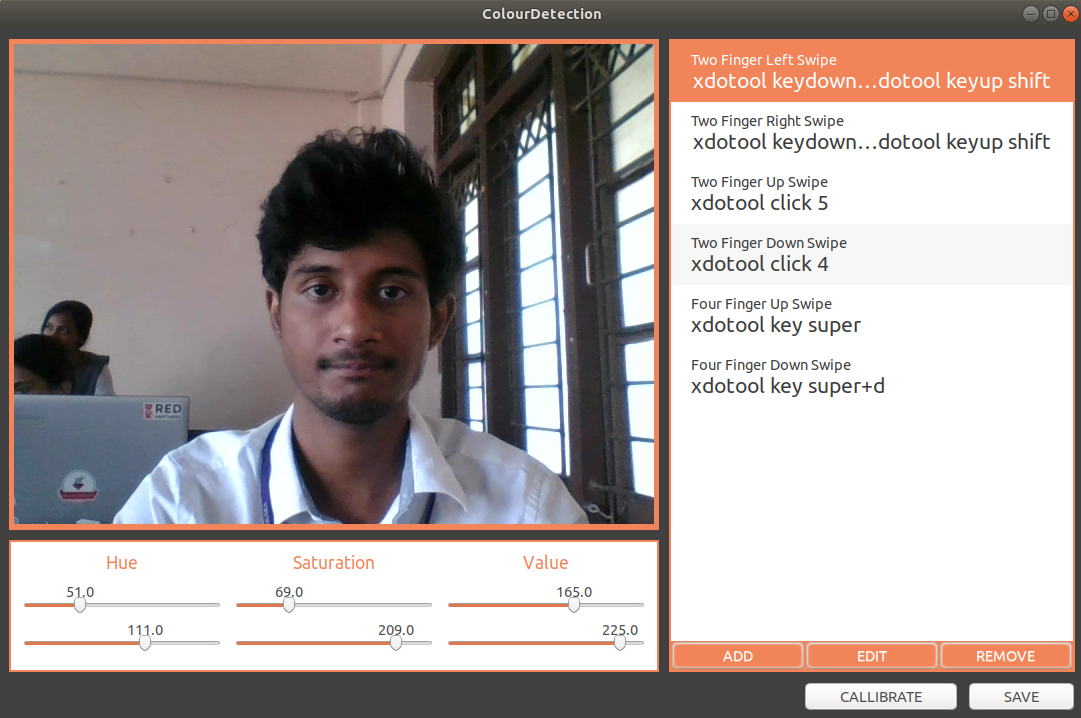
\includegraphics[width=14cm]{1.png}
    \label{Calibrate Detection}
    \caption{Calibrate Detection}
    \end{figure}

    \begin{figure}[H]
        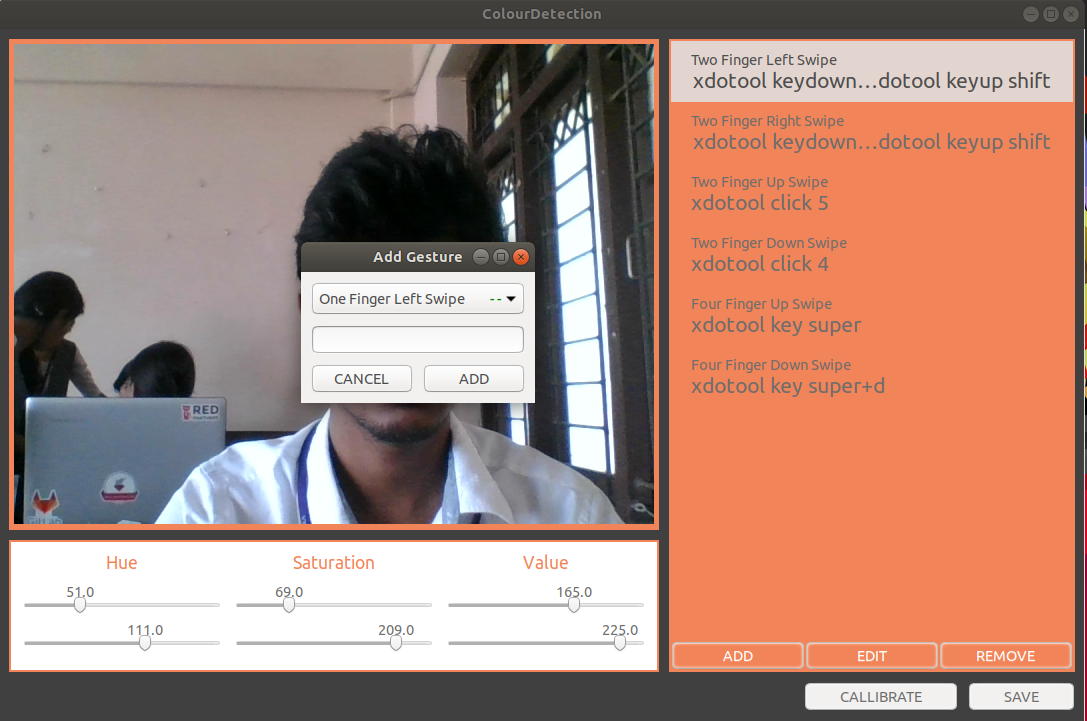
\includegraphics[width=14cm]{2.png}
        \label{Add Gesture}
        \caption{Add Gesture}
        \end{figure}

    \begin{figure}[H]
            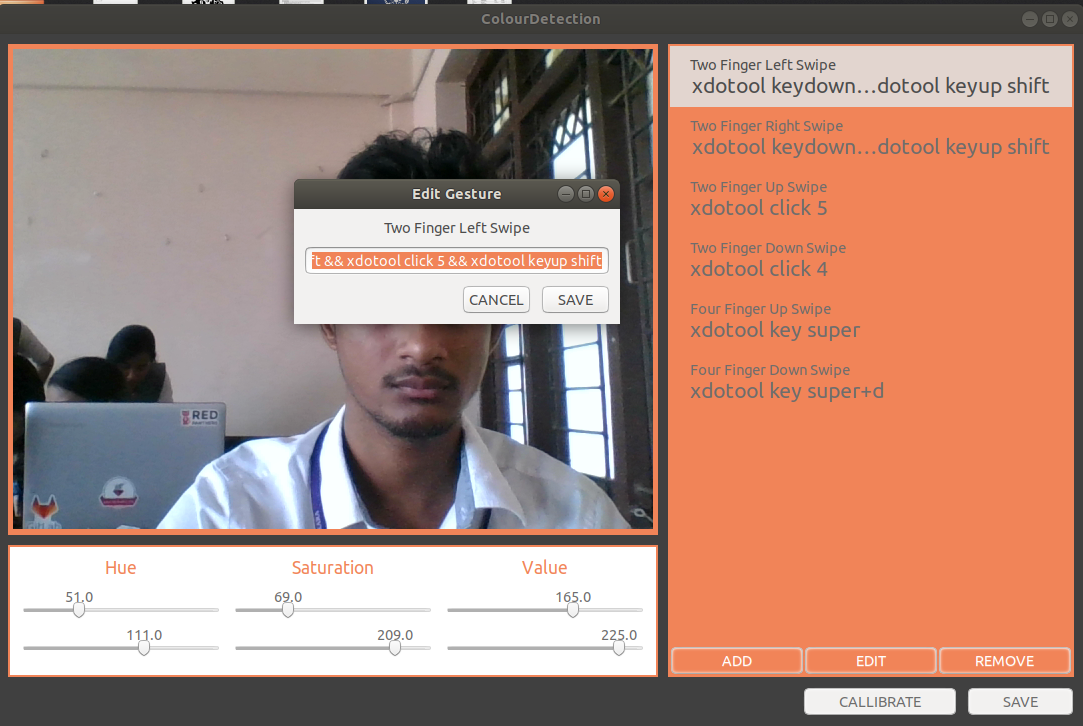
\includegraphics[width=14cm]{3.png}
            \label{Remove Gesture}
            \caption{Remove Gesture}
            \end{figure}

    \begin{figure}[H]
                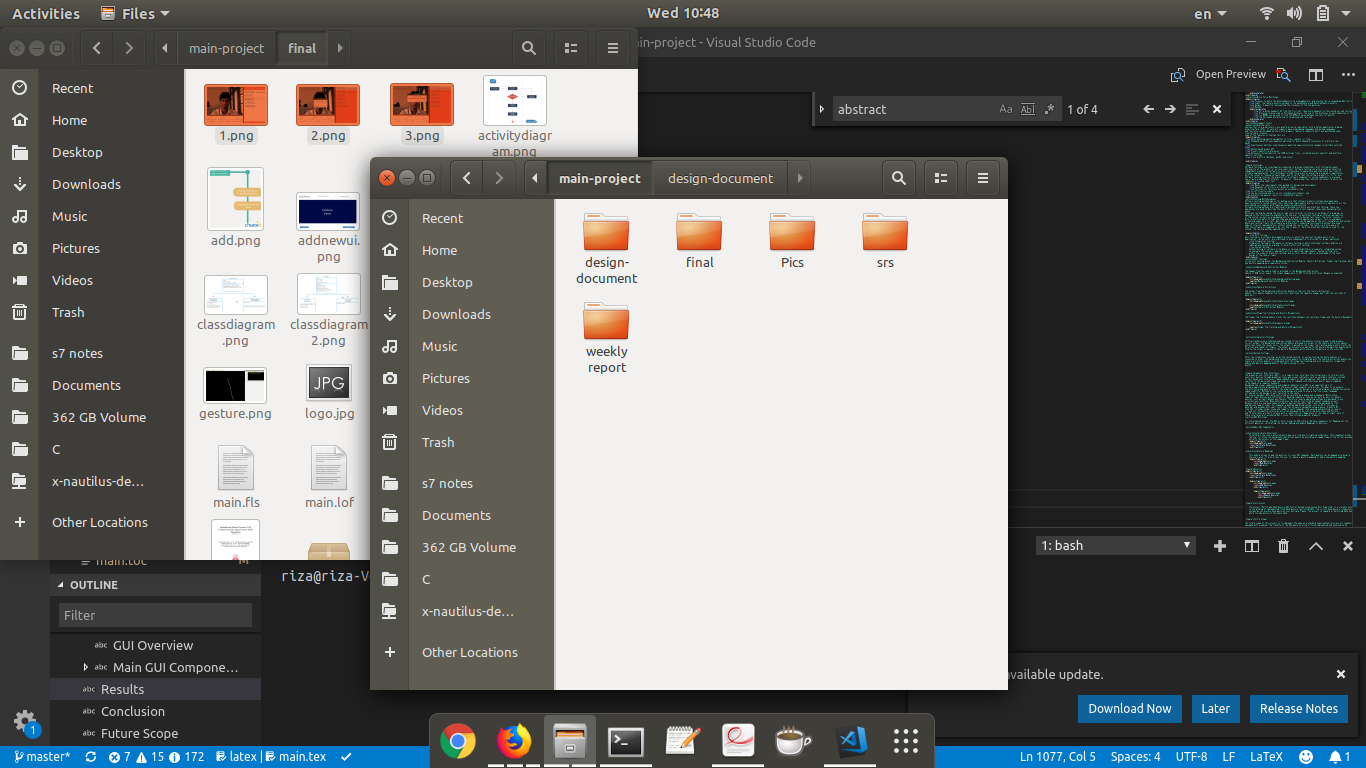
\includegraphics[width=14cm]{4.png}
                \label{Executed Gesture 4 Finger Up swipe - a}
                \caption{Executed Gesture 4 Finger Up swipe - a}

                \end{figure}
    \begin{figure}[H]
                    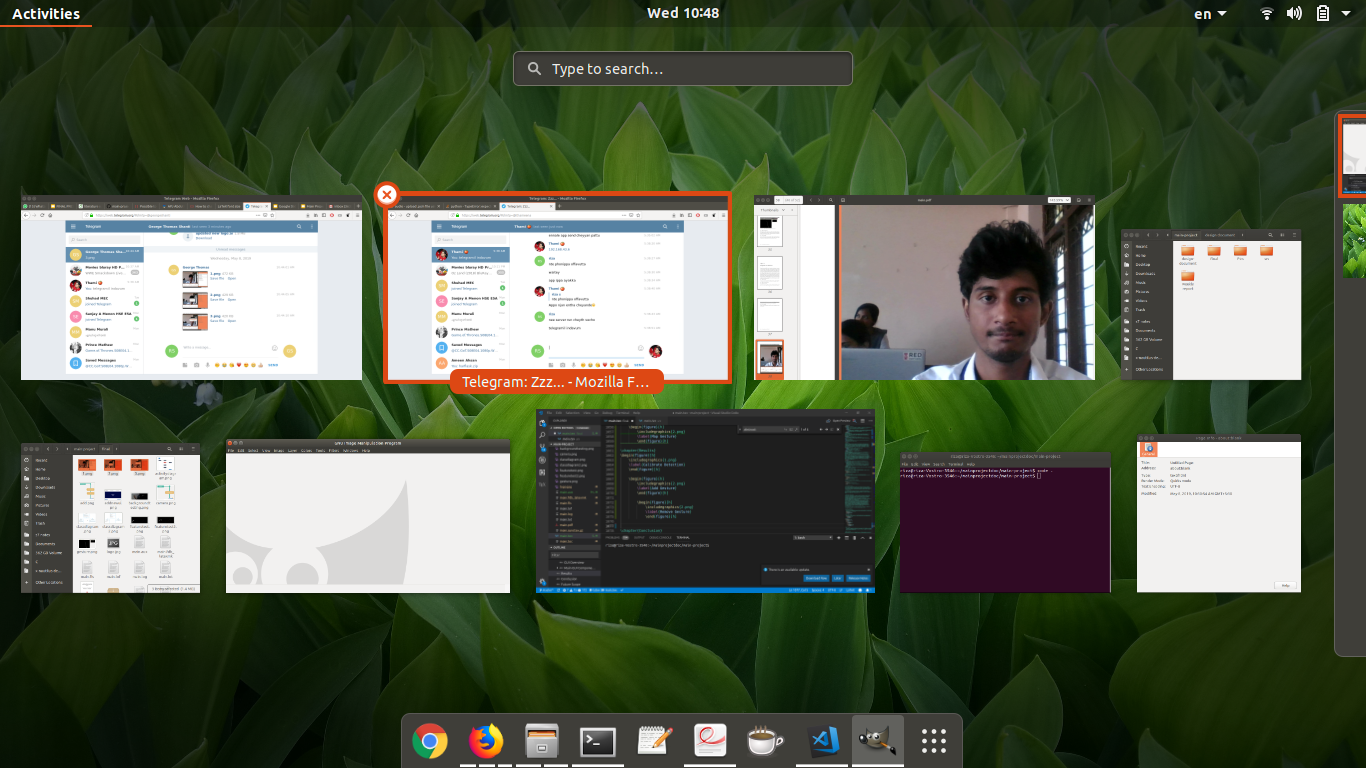
\includegraphics[width=14cm]{5.png}
                    \label{Executed Gesture 4 Finger Up swipe - b}
                    \caption{Executed Gesture 4 Finger Up swipe - b}
                    \end{figure}
\chapter{Conclusion}

    The project "MultiFrame Hand Gesture GUI Control System using Convex Hull Algorithm" is a scalable solution
    to the problem of implementing fluid Hand gesture controlled GUIs. The current Hand Gesture recognition
    systems do not process hand gestures over multiple frames. The project is capable of detecting Hand Guestures
    which include motion of the whole hand.


\chapter{Future Scope}

The future scope of this project is to implement the same as a standard input method in across all computers
equipped with a webcam. The fluidity of the GUI gestures allow it to be implemented and used easily by 
all people across the world. The hand gestures are language independant, and thus can be ported to other regions easily.

% \chapter{Publication}
   
\begin{thebibliography}{999}
\addcontentsline{toc}{chapter}{References}

    \bibitem{} K. Oka, Y. Sato, “Real-Time Fingertip Tracking and Gesture Recognition,” IEEE Computer Graphics and Applications, pp. 64-71, 2002
    \bibitem{} Lai, H. Y., Lai, H. J. (2014). Real-Time Dynamic Hand Gesture Recognition. 2014 International Symposium on Computer, Consumer and Control. 
    
    \bibitem{} Z. Ren, J. Yuan, Member, IEEE, J. Meng, Member, IEEE, and Z. Zhang, Fellow, IEEE “Robust Part-Based Hand Gesture Recognition Using Kinect Sensor,” IEEE Transactions On Multimedia, vol. 15, pp. 1110-1120, AUGUST, 2013.
    
    \bibitem{} Ji-Hwan Kim, Student Member, IEEE, Nguyen Duc Thang,Tae-Seong Kim, Member, IEEE Department of Biomedical Engineering,Department of Computer Engineering,Kyung Hee University,3-D Hand Motion Tracking and Gesture Recognition
    Using a Data Glove, IEEE International Symposium on Industrial Electronics (ISlE 2009) Seoul Olympic Parktel, Seoul, Korea July 5-8, 2009
    
    \bibitem{} Takuro Niidome, Div. of Elec. and Comp. Eng,Yokohama National University,Rokuya Ishii, Div. of Elec. \& Comp. Eng., Yokohama National University, A GUI Support System for a Sight Handicapped Person By Using Hand Shape Recognition, IECONO1: The 27th Annual Conference of the IEEE Industrial Electronics Society, 2001
    
    \bibitem{} X. Wu, C. Yang, Y. Wang, H. Li, and S. Xu, “An Intelligent Interactive System Based on Hand Gesture Recognition Algorithm and Kinect,” Fifth International Symposium on Computational Intelligence and Design, pp.294-298, 2012
    
    \bibitem{} Hayato Takahashi, Yuhki Kitazono, Integration of Hand Gesture and Multi Touch Gesture with Glove Type Device, 2016 4th Intl Conf on Applied Computing and Information Technology/3rd Intl Conf on Computational Science/Intelligence and Applied Informatics/1st Intl Conf on Big Data, Cloud Computing, Data Science \& Engineering
    
    \bibitem{} Hamid A. Jalab, Herman .K. Omer, Human Computer Interface Using Hand Gesture Recognition Based On Neural Network, 2015 5th National Symposium on Information Technology: Towards New Smart World (NSITNSW).
    
    \bibitem{} Mykyta Kovalenko, Svetlana Antoshchuk, Juergen Sieck, Real-Time Hand Tracking and Gesture Recognition Using Semantic-Probabilistic Network, 2014 UKSim-AMSS 16th International Conference on Computer Modelling and Simulation
    
    \bibitem{} Yee Yong Pang, Nor Azman Ismail, Phuah Leong Siang Gilbert, A Real Time Vision-Based Hand Gesture Interaction, 2010 Fourth Asia International Conference on Mathematical/Analytical Modelling and Computer Simulation
    



\end{thebibliography}





\end{document}
